\section{Introduction}
Nowadays, many tasks can be done by machine perception systems and learning from only a few samples has raised wide attention due to the scarcity of samples in some particular areas. Although some few-shot learning problems has almost been solved, it is still hard to achieve image detection with few training samples, the detection results are still unideal.

In the prior works, people have tried to achieve few-shot image detection by two approaches
\begin{enumerate}
    \item Meta-learning. This approach tries to transfer knowledge learnt from data-abundent classes to data-scarce novel classes so that the model could adapt to the new task more quickly. This method have been used in few-shot image classification for a while but it has not been proved effective in object detection task, which is much more challenging than image classification.
    \item Metric-learning. This approach tries to build some metrics for the learner so that it can estimate and check the similarities between images, e.g. cosine similarities. Based on the built metrics, the model can try to fit to the input and learn how to detect objects. However, this approach relis on the metric, which may be hard to find a better one.
\end{enumerate}

The object detection task is much harder than the image classification task, since it contains not only classification but also object localization. Researchers ~\cite{kang2019few,yan2019meta} have attempted to achieve few-shot object detection task, where a few labeled data, far from abundent, is provided to the learner as novel training data. These methods achieved out-of-random performance but their methods are not stable, which means the reproduced results might be far from their reported results.

\begin{figure*}[ht]
    \centering
    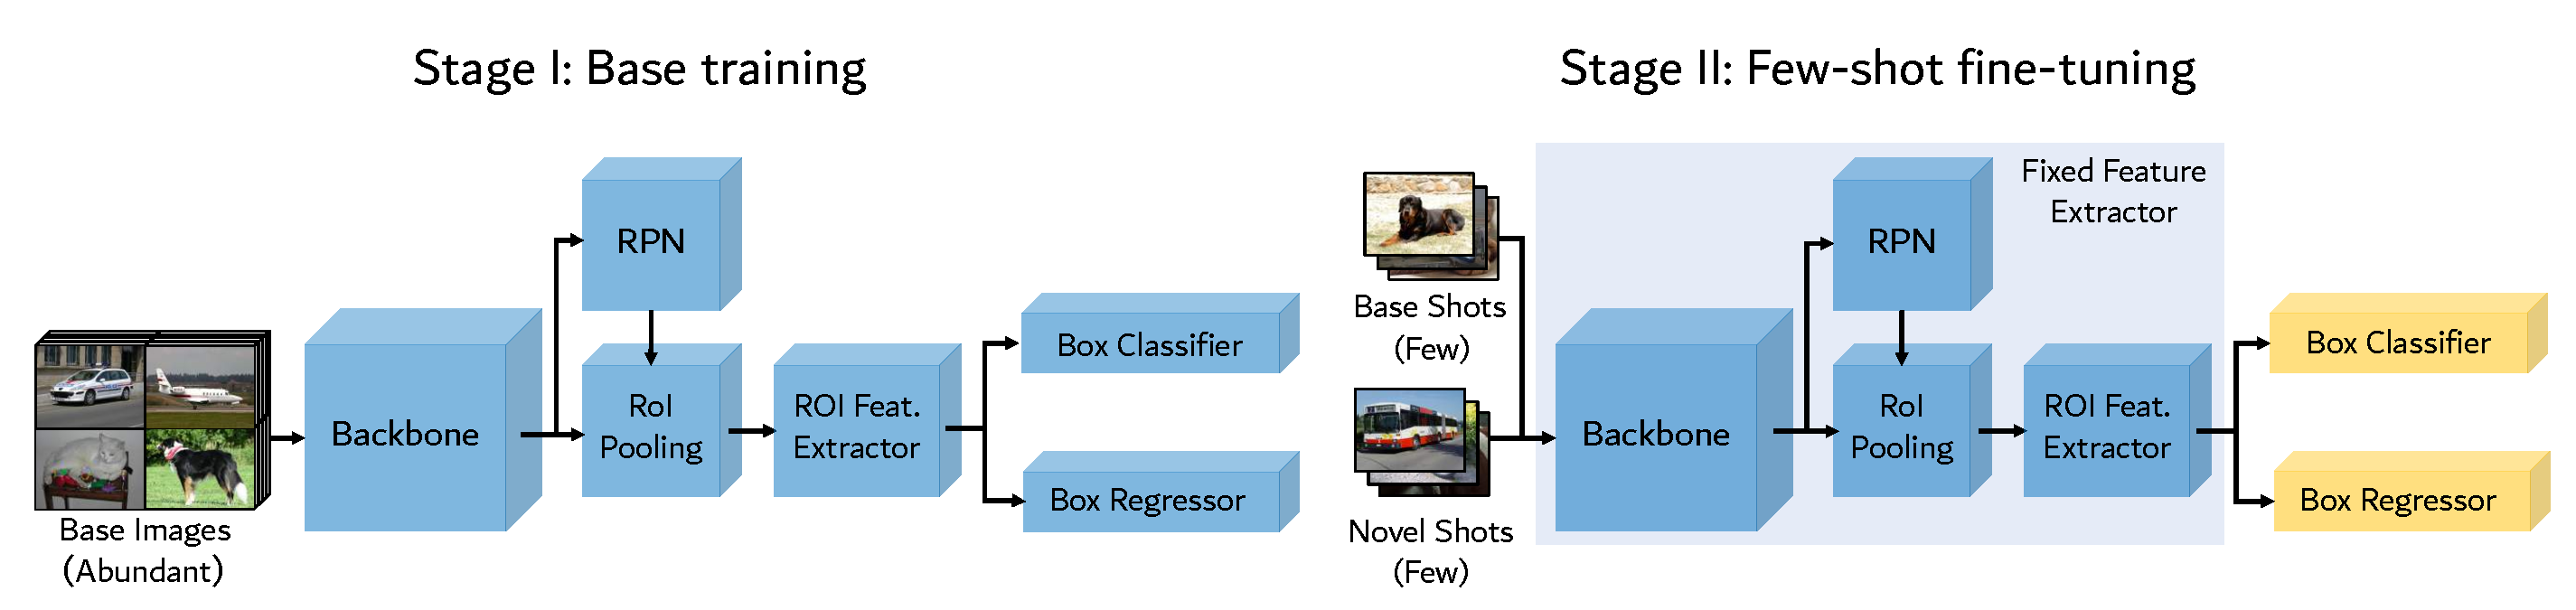
\includegraphics[width=\linewidth]{figs/TFA_fig1.pdf}
    \label{fig:tfa_arch}
    \vspace{-0.8cm}
    \caption{The two-stage fine-tuning approach (\model). In the base training stage, the entire object detector are jointly trained on the base classes. In the second stage, the labeled feature extractor is kept intact and only the last layer, i.e. box predictor, is fine-tuned on a balanced set consisting sampled base and novel classes.}
\end{figure*}

In this project, we try to improve the detection results by adopting fine-tuning based approaches. We focus on the schedule of the training procedure and use proper instance-level feature normalization in this project.

The training is composed of two stages, which is shown in Figure~\ref{fig:tfa_arch}. The first stage trains the whole network, e.g. Faster R-CNN, on data-abundent base classes. Then we only train the last layer of the network in the second stage, on a small balanced training set that is composed of both base and novel classes by properly sample data, parameters in other layers of the detector is kept intact during the second stage. We also use instance-level feature normalization in the second stage, which helps the model to diminish some parameter issues introduced by~\citet{gidaris2018dynamic}.

In our evalution, we find that our method outperfroms all previous few-shot object detection methods, our method can gain 2 $\sim$ 15 percent more accuracy than prior methods, and it even doubled the accuracy in one-shot learning, which dictates the effiction of our method.

We fixed several issues in the existing training procedures
\begin{enumerate}
    \item We try to diminish overfitting by invoking multiple runs on different random samples so that the variance is lower and the results much are more stable.
    \item We try to keep the accuracy of our method consistent with the paper.
    \item We report not only the accuracy for novel classes, but also accuracy for base classes and the overall accuracy for all classes, so that one can see that the accuracy (referred to as the generalized few-shot learning setting in the few-shot classification literature~\cite{hariharan2017low,wang2019tafe}) for other classes are not largely affected.
\end{enumerate}
